\documentclass[a4paper,norsk, 10pt]{article}
\usepackage[utf8]{inputenc}
\usepackage{verbatim}
\usepackage{listings}
\usepackage{graphicx}
\usepackage[norsk]{babel}
\usepackage{a4wide}
\usepackage{color}
\usepackage{amsmath}
\usepackage{float}
\usepackage{amssymb}
\usepackage[dvips]{epsfig}
\usepackage[toc,page]{appendix}
\usepackage[T1]{fontenc}
\usepackage{cite} % [2,3,4] --> [2--4]
\usepackage{shadow}
\usepackage{hyperref}
\usepackage{titling}
\usepackage{marvosym }
\usepackage{subcaption}
\usepackage[noabbrev]{cleveref}
\usepackage{cite}


\setlength{\droptitle}{-10em}   % This is your set screw

\setcounter{tocdepth}{2}

\lstset{language=c++}
\lstset{alsolanguage=[90]Fortran}
\lstset{alsolanguage=Python}
\lstset{basicstyle=\small}
\lstset{backgroundcolor=\color{white}}
\lstset{frame=single}
\lstset{stringstyle=\ttfamily}
\lstset{keywordstyle=\color{red}\bfseries}
\lstset{commentstyle=\itshape\color{blue}}
\lstset{showspaces=false}
\lstset{showstringspaces=false}
\lstset{showtabs=false}
\lstset{breaklines}
\title{FYS2130 Oblig 1}
\author{Daniel Heinesen, daniehei}
\begin{document}
\maketitle

\section*{Forståelses- og diskusjonsspørsmål.}

\subsection*{2)}
For å få svingninger må kraften være en funksjon av posisjon og hastighet. Kraften må også bytter retning om et likevektspunkt. Vi kan da sette opp en differensiallikning som gir et svar på formen $x(t) = \mathcal{D}e^{i\theta}$

\subsection*{4)}
Perioden til en svigning er gitt ved

\begin{equation}
T = \frac{2\pi}{\omega}
\end{equation}

For en fjær og et lodd er vinkelfrekvensen gitt som

$$
\omega = \sqrt{\frac{k}{m}}
$$

Perioden er derfor bare en funksjon av massen $m$ og fjærstivheten $k$, og siden begge disse er like på månen som på jorden, vil ikke perioden endres.

\subsection*{5)}

I forelesningen fant vi at for en pendel er vinkelfrekvensen $\omega$ gitt som

$$
\omega = \sqrt{\frac{g}{L}}
$$


Og perioden er dermed

$$
T = 2\pi \sqrt{\frac{L}{g}}
$$

Siden gravitasjonskonstanten, $g$ på månen er ca $1/6$ av den på jorden vil perioden på månen være ca $\sqrt{6}$ ganger høyere enn på jorden.

\subsection*{7)}

Om en fjær komprimeres eller strekkes for mye vil den ikke i dette domenet ikke følge Hooks lov. Har man feks en for stor masse, vil fjæren trekkes for langt, og bevegelsen blir ikke lenger harmonisk.

\newpage

\section*{Regneoppgaver.}
\subsection*{9)}

For et lodd som henger i en fjær gjelder bevegelseslikningene:

$$
x(t) = A\cos(\omega t + \phi)
$$
$$
v(t) = -A\omega \sin(\omega t + \phi)
$$

Plotter vi dette mot hverandre med $\omega = A = 1$ og $\phi = 0$ får vi:

\begin{figure}[H]
\centering

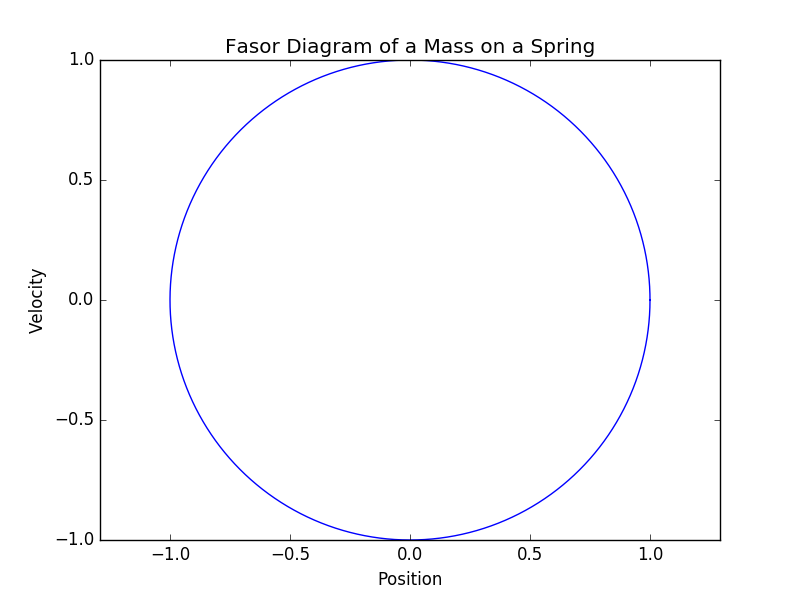
\includegraphics[scale=0.5]{springFasor.png}
\caption{Fasordiagrammet til et lodd hengende på en fjær.}
\end{figure}

Diagrammet ser ut som en sirkel med radius $A = 1$. 


\subsection*{10)}
Bevegelsen til en ball som spretter opp og ned følger:

$$
x(t) =s_0 + v_0t + \frac{1}{2}gt^2
$$
$$
v(t) = v_0 + gt
$$

Vi bruker at $s_0 = 0$, $v_0 = 1$ og $g = -9.81$. Vi får da plottet:

\begin{figure}[H]
\centering

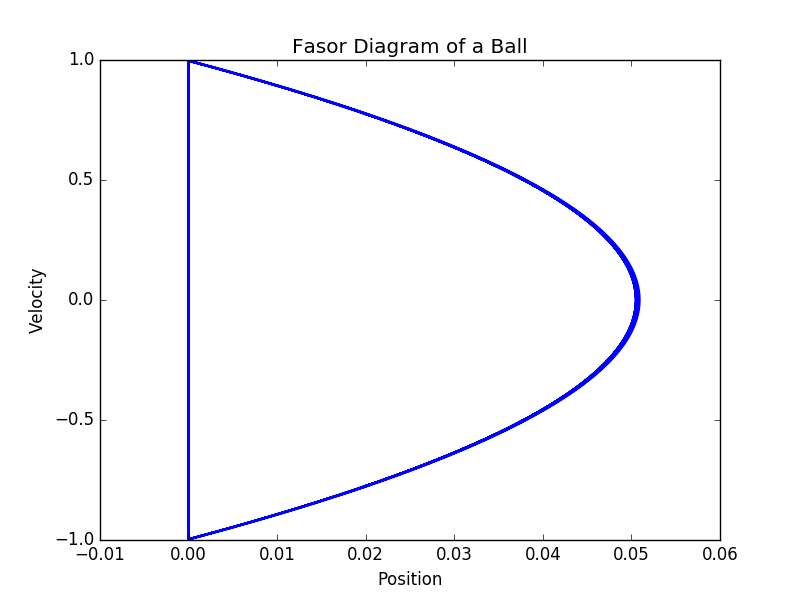
\includegraphics[scale=0.5]{ballFasor.png}
\caption{Fasordiagrammet til en sprettende ball.}
\end{figure}

Selv om dette er en sprettende ball ser det ut som en ball som blir kastet opp og faller ned til bakken. Dette er fordi baller spretter elastisk og banene til banen er helt like. Dette er derfor en periodisk bevegelse. I motsetning til loddet er ikke dette fasor diagrammet sirkulert. Dette er fordi hastigheten ikke er kontinuelig, siden kraften er konstant, unntatt når 

Diagrammet er ganske ulikt det for loddet. Dette er fordi kraften på ballen er kostant over mesteparten av banen, annet enn når ballen spretter i bakken, hvor det er en fjærkraft med $k = 10^{10}$. I diagrammet ser hastigheten nesten inkontinuelig ut, men der ballen spretter ser diagrammet ut som en avlang versjon av det for loddet:

\begin{figure}[H]
\centering

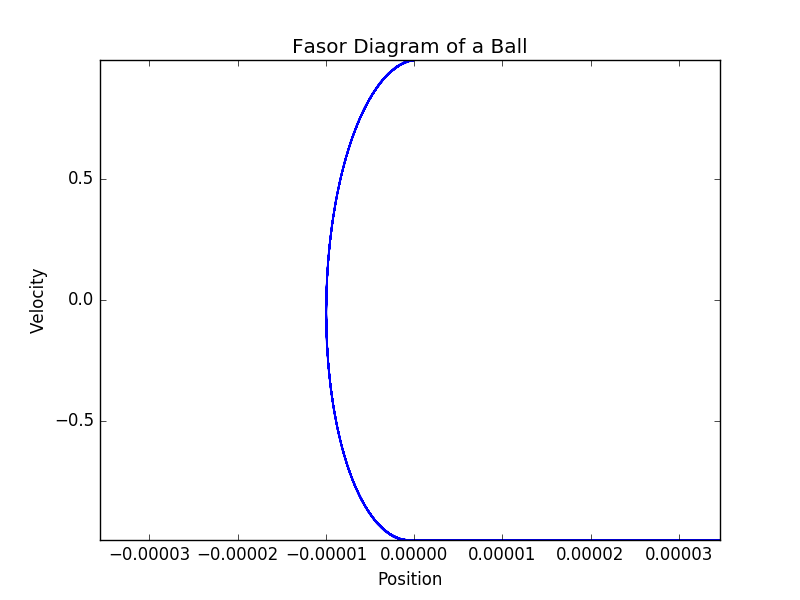
\includegraphics[scale=0.5]{ballSprett.png}
\caption{Fasordiagrammet til en sprettende ball zoomet inn i der ballen spretter}
\end{figure}

\subsection*{11)}
Vi vet at fjæren har likevektspunktet $0.3m$ før loddet er festet, og $0.48$ etter. Dette betyr at fjæren har strukket seg $-0.18m$. Loddet veier $0.1kg$. Vi kan så bruke Newtons første lov $F = 0$:

$$
-kx-mg = -k(-0.18) -mg = 0
$$

$$
k = \frac{mg}{0.18} = 5.45
$$

Vi kan så finne perioden fra dette:

$$
T = 2\pi \sqrt{\frac{m}{k}} = 0.85 sek
$$

Vi kan nå bruke bevegelseslikningene til et lodd i en fjær:

$$
x(t) = A\cos(\omega t + \phi)
$$
$$
v(t) = -A\omega \sin(\omega t+ \phi)
$$

Vi evaluere så disse for punket hvor fjæren slippen. Vi vet at her er:

$$
x(t=0) = A\cos(\phi) = -0.08 m
$$

$$
v(t=0) = -A\omega \sin(\phi) = 0
$$

Deler vi disse på hverandre får vi at

$$
\frac{v(0)}{x(0)} = -\omega \tan(\phi) = 0
$$

Dette sier oss at $\phi = 0$. Setter vi dette inn i linkenen for posisjon, finner vi at $A = x_0 = -0.08 m$. Siste vi trenger å finner er at:

$$
\omega = \sqrt{\frac{k}{m}} = 7.38
$$

M.a.o beveger dette systemet seg etter:

$$
x(t) = -0.08\cos(7.38t)
$$

Siden $\phi = 0$, vil det maksimale/minimale utslaget, og dermed kraften finne sted i $x = \pm A$. Så den maksimale/minimale kraften er

$$
F = \pm kx = \mp 5.45\cdot 0.08 = \mp 0.44 N
$$

\subsection*{12)}

Vi har at $f = \frac{1}{T} = 0.4 Hz$. Dette gir oss at $\omega = \frac{2\pi}{T} = 2\pi f = \frac{4\pi}{5}$. For å finne akselerasjonen, bruker vi at den er gitt ved:

$$
a = -\frac{kx}{m}
$$

$$
\frac{k}{m} = -\frac{a}{x}
$$

Vi kan sette dette inn for $\omega$:

$$
\omega = \sqrt{\frac{k}{m}} = \sqrt{\frac{-a}{x}} = 2\pi f
$$

$$
\Rightarrow a(x) = -(2\pi f)^2x
$$

Vi kan så finne akselerasjonen for $t=2.0$. Vi vet at $x(t) = 0.024m$,så

$$
a(0.024) = -0.1516 m/s^2
$$

Vi kan nå bruke de 3 bevegelseslinknene:

$$
x(t=2) = A\cos(\omega\cdot 2s + \phi) = 0.024m
$$
$$
v(t=2) = -A\omega \sin(\omega\cdot 2s + \phi) = -0.16 m/s
$$
$$
a(t=2) = -A\omega^2 \cos(\omega \cdot 2s + \phi) = -0.1516 m/s^2
$$

Vi ønsker å finne $\phi$, vi tar da og:

$$
\frac{v}{a} = \frac{1}{\omega}\tan(\omega \cdot 2s + \phi) = \frac{0.16}{0.1516} = 1.06
$$
$$
\phi = \arctan(1.05\omega) - \omega \cdot 2s = -3.82 rad = 2.47 rad
$$

 Vi kan nå enkelt finne $A$

$$
x = A\cos(\omega\cdot 2s + 2.47) = 0.024m \Rightarrow A = 0.068m = 6.8cm
$$

Vi får da at svigningen følger:

$$
x(t) = 0.068\cos[\frac{4\pi}{5}t + 2.47]
$$

\subsection*{13)}
For et lodd i en fjær er kinetisk energi $E_k$ og potentiell energi $E_p$ gitt som:

\begin{equation}
E_k = \frac{1}{2}m \dot{x}^2
\end{equation}\label{eq:ek}

$$
= \frac{1}{2}A^2 \omega^2 \sin^2(\omega t) 
$$

\begin{equation}
E_p = \frac{1}{2}kx^2
\end{equation}\label{eq:ep}

$$
= \frac{1}{2}kA^2 \cos^{2}(\omega t)
$$

Vi ønsket å finne $x(t)$ når $E_k = \frac{1}{2} E_p$:

$$
E_k = \frac{1}{2} E_p
$$

$$
\frac{1}{2}mA^2 \omega^2 \sin^2(\omega t)  = \frac{1}{4}kA^2 \cos^{2}(\omega t)
$$

$$
\Rightarrow \tan^2(\omega t) = \frac{k}{2m\omega^2} \Rightarrow t = \frac{1}{\omega} \arctan \frac{\sqrt{k}}{\sqrt{2m}\omega}
$$

Setter vi nå dette inn i $x(t) = A\cos(\omega t)$ får vi at

$$
x = A\cos(\omega \frac{1}{\omega} \arctan \frac{\sqrt{k}}{\sqrt{2m}\omega}) = A\cos(\arctan(\frac{\sqrt{k}}{\sqrt{2m}\omega}))
$$

Vi kan så bruke identiteten at

$$
\cos(\arctan(x)) = \frac{1}{\sqrt{x^2 + 1}}
$$

og får

$$
x = \frac{A}{\sqrt{\frac{k}{2m\omega ^2}+1}} = \frac{A}{\sqrt{\frac{1}{2}+1}} = 0.816A
$$

\subsection*{14)}
Systemet beveger seg etter:

$$
z(t) = A\cos(\omega t + \phi)
$$

Hvor $A = 1.2m$, $\omega = 2\pi f = 6\pi$ og $\phi = \frac{\pi}{6}$.
\subsubsection*{a)}
Vi kan skrive om $z(t)$:

$$
z(t) = A\cos(\omega t + \phi) = A\{\cos(\omega t)\cos(\phi) - \sin(\omega t)\sin(\phi)\}
$$

Setter vi at $B = A\cos(\phi) = 1.04m$ og $C = -A\sin(\phi) = -0.6m$ får vi at

$$
z(t) = 1.04\cos(6 \pi t) - 0.6\sin(6\pi t)
$$


\subsubsection*{b)}
Vi kan også skrive:

$$
z(t) = A\cos(\omega t + \phi) = \mathcal{R}\{A(\cos(\omega t + \phi) + \i \sin(\omega t + \phi))\} = \mathcal{R}\{Ae^{i(\omega t + \phi)}\}
$$

$$
z(t) = \mathcal{R}\{1.2e^{ i (6\pi t + \frac{\pi}{6})}\}
$$

\subsection*{15)}

$$
z(t) = A\sin(\omega t) + B\cos(\omega t) 
$$

Hvor $A = 1.2m$, $B = 0.7m$ og $\omega = 6\pi$. Vi vet fra forrige oppgave at vi 

$$
A = -C\sin(\phi)
$$
$$
B = C\sin(\phi)
$$

Vi ønsker å finne $C$ og $\phi$.

$$
A^2 + B^2 = C^2(\cos^2(\phi) +\sin^2(\phi)) = C^2 
$$

$$
\frac{A}{B} = \frac{-\sin(\phi)}{\cos(\phi)} = -\tan(\phi)
$$

Så

$$
C = \sqrt{A^2 + B^2} = 1.39m
$$
$$
\phi = \arctan(\frac{A}{B}) = 1.04 \approx \frac{\pi}{3}
$$


Vi kan derfor skrive:

$$
z(t) = A\sin(\omega t) + B\cos(\omega t) = C\cos(\omega t + \phi) = 1.39\cos(6\pi t + \frac{\pi}{3})
$$

\subsection*{16)}
Vi øsnker å skrive $y(t)$ så generelt som mulig, for å gjøre det enklere å drive med algebraen:

$$
y(t) = \mathcal{R}\{ (-5.8 + 2.2i)e^{i\omega t}  \} = \mathcal{R}\{ (a + bi)e^{i\omega t}  \} 
$$

Vi kan så begynne å manipulere uttrykket ved å bruke Eulers formel:

$$
\mathcal{R}\{ (a + bi)e^{i\omega t}  \}  = \mathcal{R}\{ ae^{i\omega t} +ib e^{i\omega t}\} = \mathcal{R}\{ a\cos(\omega t) + ai\sin(\omega t) + b\cos(\omega t) + ib\cos(\omega t) - b\sin(\omega t) \} 
$$

$$
= a\cos(\omega t) - b\sin(\omega t) = -5.8\cos(\omega t) - 2.2\sin(\omega t)
$$

Vi vil nå gjøre det om det om på formen $y(t) = C\cos(\omega t + \phi)$. Om vi ser at $A = -5.8$ og $B = -2.2$. Kan vi finne at:

$$
C = \sqrt{A^2 + B^2} = 6.203 m
$$

og

$$
\phi = -\arctan(\frac{A}{B}) = -1.208
$$


Så vi får da at:

$$
y(t) = 6.203\cos(\omega t - 1.208)
$$

\subsection*{19)}

Den totale energien er definert som $E = E_k + E_p$, hvor $E_k = \frac{1}{2}m\dot{x}^2 = \frac{1}{2}ml^2\dot{\theta}^2$, hvor $l$ er lengden til pendelen, og $E_p = mgh = mgl\cos(\theta)$. Vi finner da at

$$
\frac{dE}{dt} = \frac{dE_k}{dt} + \frac{dE_p}{dt} = \frac{d(\frac{1}{2}ml^2\dot{\theta}^2)}{dt} + \frac{d(mgl\cos(\theta))}{dt}
$$

$$
= ml^2\dot{\theta}\ddot{\theta} - mgl\sin(\theta)\dot{\theta}
$$

Her ble produkt regelen brukt. Vi trenger så å bruke kraften $F = -b\dot{x} +mg\sin(\theta) = m\ddot{x}$ for å finne at

$$
\ddot{x} = -\frac{b\dot{x}}{m} + \frac{mg\sin(\theta)}{m}
$$

Men vi er interessert i $\ddot{\theta}$ som er gitt ved:

$$
\ddot{\theta} = \frac{\ddot{x}}{l} = -\frac{b\dot{x}}{lm} + \frac{gl\sin(\theta)}{l} = -\frac{b\dot{\theta}l}{lm} + \frac{gl\sin(\theta)}{l} =- \frac{b\dot{\theta}}{m} + \frac{g\sin(\theta)}{l}
$$

Vi får da at:

$$
\frac{dE}{dt} = ml^2\dot{\theta}\ddot{\theta} + mgl\sin(\theta)\dot{\theta} = ml^2\dot{\theta}(- \frac{b\dot{\theta}}{m} - \frac{g\sin(\theta)}{l}) + mgl\sin(\theta)\dot{\theta}
$$

$$
= -bl^2\dot{\theta}^2 - mgl\sin(\theta)\dot{\theta} + mgl\sin(\theta)\dot{\theta} = -bl^2\dot{\theta}^2 = -bv^2
$$

Så vi har besvist at 

$$
\frac{dE}{dt} = -bv^2
$$






\end{document}


